\newpage
\section{Lower Bound}
下界和问题有关. 算法复杂度不可能小于下界. 若复杂度达到下界, 算法就是最优的. 但即使算法是最优的, 也可能复杂度大于下界. 

Techniques:
\begin{itemize}
    \item decision tree
    \item Adversary(Oracle)
\end{itemize}

\subsection{Adversary Argument(Oracle)}
\begin{definition}[Adversary]
    A strategy to create situation to make the algorithm to work hard (releasing the least information and changing scenario).
\end{definition}

为问题建立最坏的情况. 


\subsection{Decision Tree}
\subsubsection{硬币称重}
以硬币称重问题为例, 就是天平可以给左倾, 右倾, 平衡三种选项. 

\begin{itemize}
    \item 给 8 个硬币, 找到一个轻的, 最少需要 $\left\lceil \log_3 8 \right\rceil=2$
    \begin{figure}[H]
        \centering
        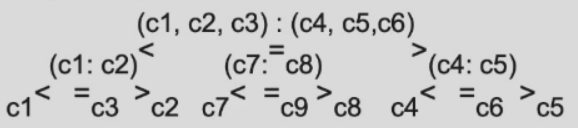
\includegraphics[width=0.42\textwidth]{pic/DAA2/8coin.png}
        \caption{8 个硬币}
    \end{figure}
    
    \item 给 12 个硬币, 找到一个重量不一样的, 最少需要 $\left\lceil \log_3 2*12 \right\rceil=3$
    \subitem 确保每次称重, 都让可能的结果减少到 $1/3$

    \begin{figure}[H]
        \centering
        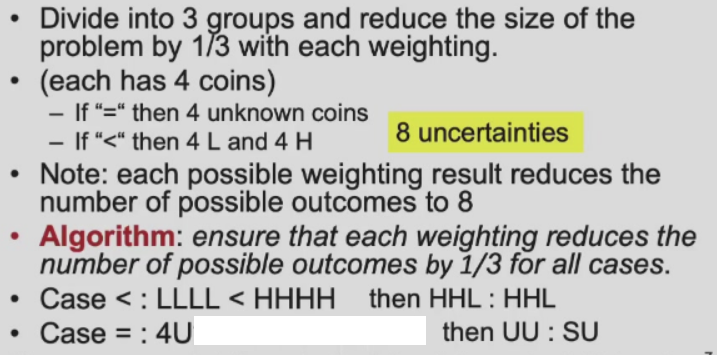
\includegraphics[width=0.309\textwidth]{pic/DAA2/12coin.png}
        \caption{12 个硬币}
    \end{figure}
    $S$ 表示 standard
\end{itemize}

\subsubsection{Finding an element in a sorted list}
给定有序序列, 找特定元素. 可以使用比较 $>=<$, 可能找不到. 下界: $\left\lceil \log_2(n+1) \right\rceil$. 

\begin{figure}[H]
    \centering
    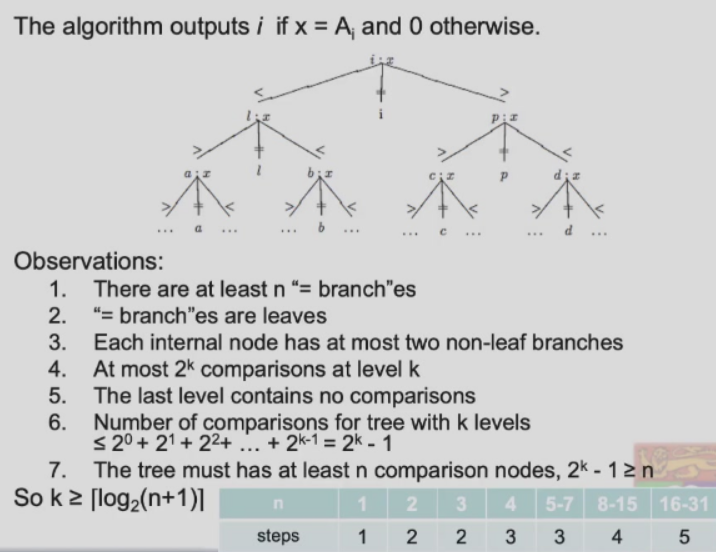
\includegraphics[width=0.42\textwidth]{pic/DAA2/sorted下界.png}
    \caption{下界推导}
\end{figure}


\subsection[Finding the Maximum and Minimum]{Finding the Maximum and Minimum of N-Elements}

\subsubsection{Divide and Conquer Approach}
\begin{figure}[H]
    \centering
    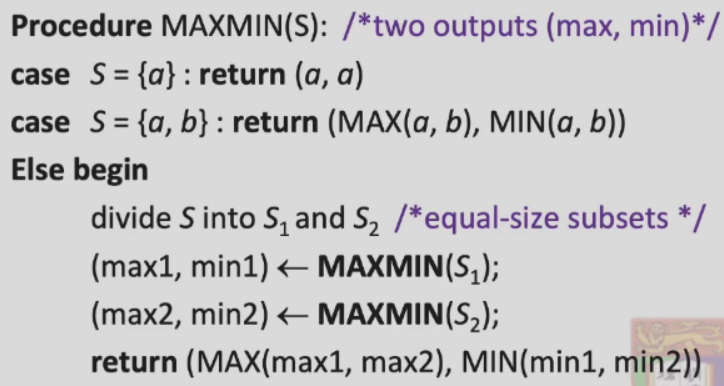
\includegraphics[width=0.42\textwidth]{pic/DAA2/Divide and Conquer Approach}
    \caption{Divide and Conquer Approach}
\end{figure}

\paragraph{Complexity}用公式推导 
\begin{align*}
    T(n)&=2T(n/2)+2\\
    &=3n/2-2
\end{align*}
where $|S|=n=2^m$


\begin{proof}[Proof by Adversary] (给予最少的信息/最多的比较)
    \begin{figure}[H]
        \centering
        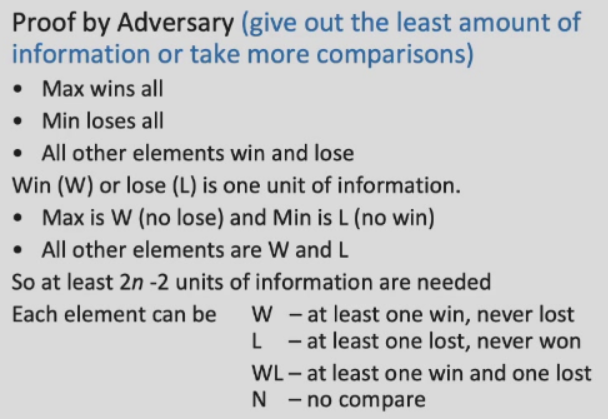
\includegraphics[width=0.42\textwidth]{pic/DAA2/Proof by Adversaryp1.png}
        \caption{Proof by Adversary}
    \end{figure}
    
    \begin{figure}[H]
        \centering
        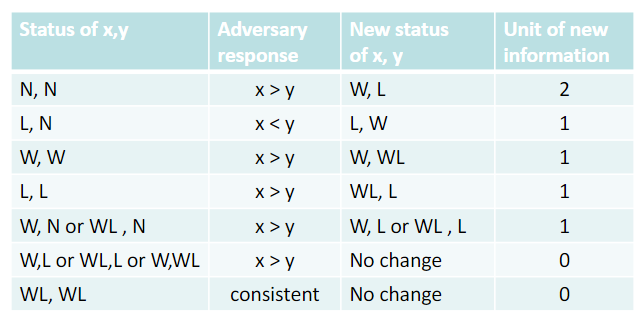
\includegraphics[width=0.309\textwidth]{pic/DAA2/Adversary strategy}
        \caption{Adversary strategy}
    \end{figure}
    最后一行是 WL, WL, 随机给结果, 不给信息.

    \begin{figure}[H]
        \centering
        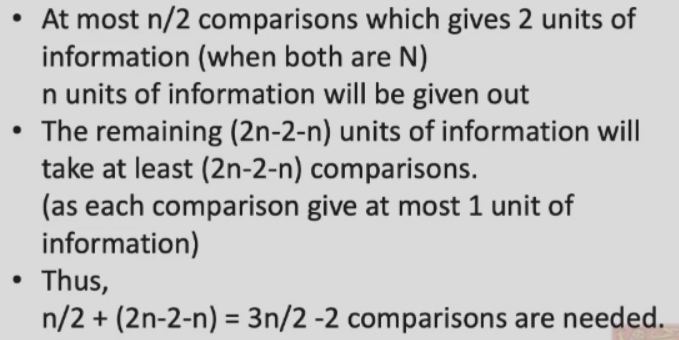
\includegraphics[width=0.309\textwidth]{pic/DAA2/Analysis}
        \caption{Analysis}
    \end{figure}
    
\end{proof}

example: 略了. 就是可以依据策略改结果. 

\subsection{Finding Second Maximum Element}
必须找到最大值才能找到次大值. 

\subsubsection{Adversary}
最大值一直 win, 让其难以找到次大值. 

\begin{figure}[H]
    \centering
    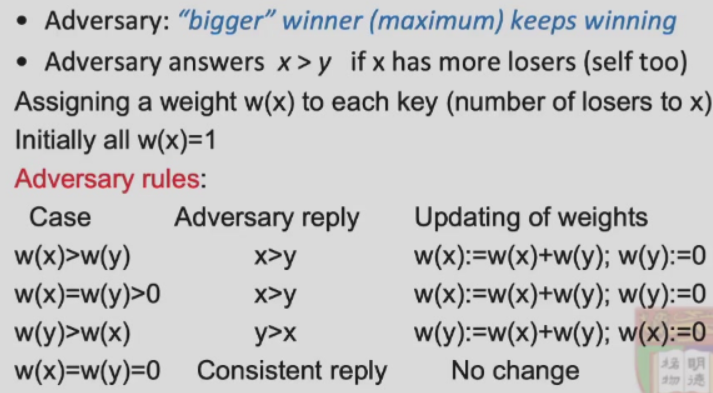
\includegraphics[width=0.309\textwidth]{pic/DAA2/Adversary}
    \caption{Adversary strategy}
\end{figure}

\subsubsection{Lower Bound}
\begin{figure}[H]
    \centering
    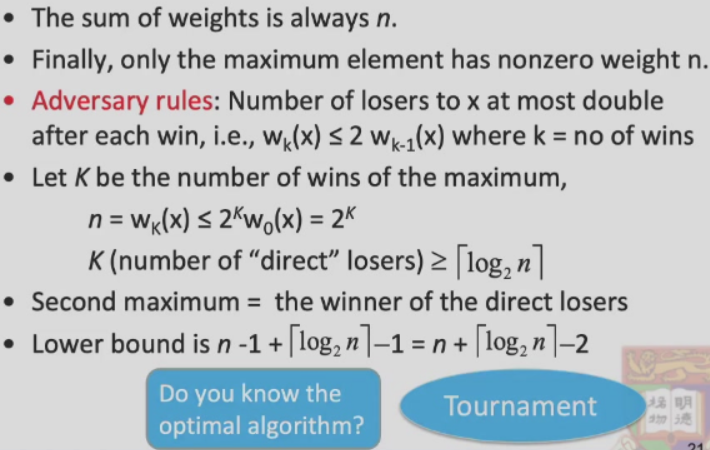
\includegraphics[width=0.42\textwidth]{pic/DAA2/Lower Bound}
    \caption{Lower Bound}
\end{figure}

\subsection{Merging Sorted Lists}
Problem: Merge two sorted lists 

\begin{figure}[H]
    \centering
    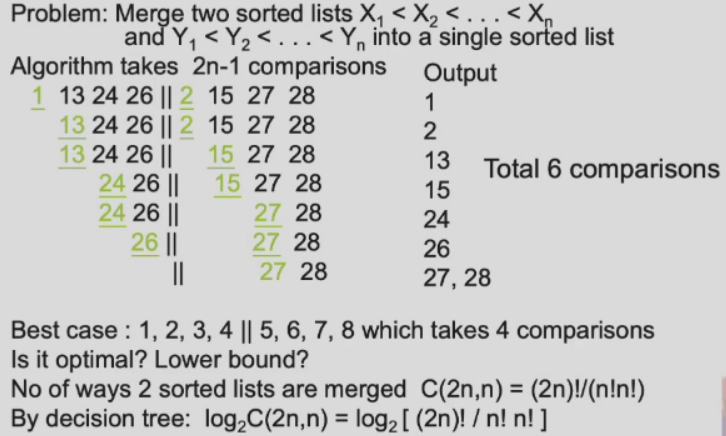
\includegraphics[width=0.309\textwidth]{pic/DAA3/Merging Sorted Lists}
    \caption{Merging Sorted Lists}
\end{figure}

\subsubsection{Adversary proof}
\begin{figure}[H]
    \centering
    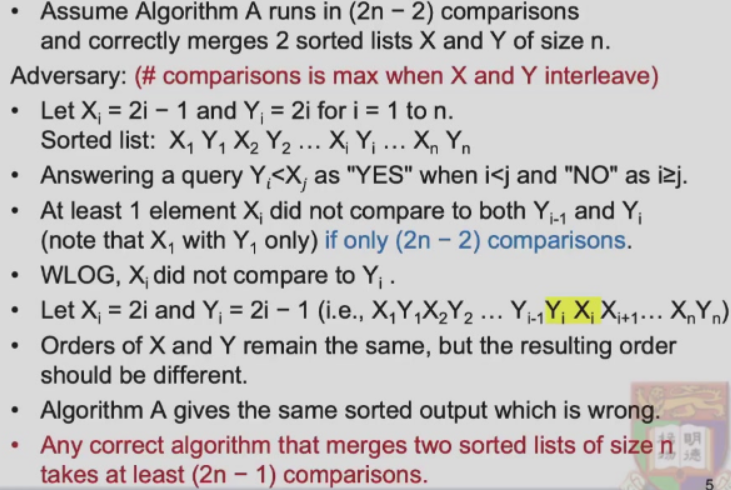
\includegraphics[width=0.309\textwidth]{pic/DAA3/Adversary proof}
    \caption{Adversary proof}
\end{figure}